%\documentclass[notes,usenames,dvipsnames]{beamer}
%\documentclass[notes]{beamer}       % print frame + notes
%\documentclass[notes=only]{beamer}   % only notes
\documentclass[usenames,dvipsnames]{beamer}             % only frames
\usepackage[outputdir=out]{minted}
\usepackage{pgfpages}
%\setbeameroption{show notes on second screen}
%\setbeameroption{show notes}
%subfigures
\usepackage{caption}
\usepackage{subcaption}

%tables packages
\usepackage{multirow}

% math
\usepackage{amsmath}

% bash command
\usepackage{graphicx}
\usepackage{listings}
% varbatim for ascii figures
\usepackage[T1]{fontenc}
\usepackage[utf8]{inputenc}
%\usepackage{verbatim}
\usepackage{lipsum} % for context
\usepackage{fancyvrb}
\usepackage{varwidth}
\usepackage{circuitikz}
\ctikzset{logic ports=ieee}
\usepackage{listings}
% \lstset{language=[Motorola68k]Assembler,basicstyle=\ttfamily,keywordstyle=\color{blue}}

\usepackage{shellesc}
\usepackage{adjustbox}

\newsavebox{\asciigcn}

% notes prefixed in pympress
\addtobeamertemplate{note page}{}{\thispdfpagelabel{notes:\insertframenumber}}
%theme used
\usetheme{Madrid}
%Information to be included in the title page:
\title[Computer Architecture] %optional
{Computer Architecture}

\subtitle{Course no. 9 - Microcoded CPU}

\author[Ștefan-Dan Ciocîrlan] % (optional, for multiple authors)
{}

\institute[NUSTPB] % (optional)
{
  \inst{}%
  National University of Science and Technology\\
  POLITEHNICA Bucharest
}

\date[NUSTPB 2025] % (optional)
{Computer Architecture}

\logo{
\includegraphics[height=0.9cm]{../../media/LOGO_UNSTPB_en.png}
\includegraphics[height=0.9cm]{../../media/logoACSQ.jpeg}
}


% Roman numerals
\newcommand*{\rom}[1]{\expandafter\@slowromancap\romannumeral #1@}
%split
\usepackage{amsmath}
%colors
%\usepackage[usenames,dvipsnames]{color} %loaded by the dcoument class
%subfigure
\usepackage{subcaption}
% block over block uncover
\setbeamercovered{invisible}
%\setbeamercovered{transparent}

%extra slide content
\AtBeginSection[]
{
  \begin{frame}
    \frametitle{Content}
    \tableofcontents[currentsection]
  \end{frame}
}
%notes or not
%\setbeamertemplate{note page}[plain]

\begin{document}

\frame{\titlepage}

\section{Microcoded Concepts}
% Slide 1: Introduction to Control Units
\begin{frame}
    \frametitle{Introduction to Control Units}
    \begin{itemize}
        \item The control unit directs CPU operations and generates control signals to execute instructions.
        \item Types of control units:
            \begin{itemize}
                \item \textbf{Unpipelined Hardwired Control Unit} (Von Neumann-style): Control signals generated directly by hardware.
                \item \textbf{Microprogrammed Control Unit} (Wilkes-style): Control signals generated by stored microinstructions.
                \item \textbf{Pipelined Hardwired Control Unit}: Adds pipeline stages for improved performance.
            \end{itemize}
        \item They aim to generate control signals,
        but they differ in implementation and use cases.
    \end{itemize}
    \note{
        This slide introduces students to the idea that control units
        play a critical role in CPU operation by generating the signals
        needed for instruction execution. We'll examine the characteristics,
        pros, and cons of two major types: unpipelined hardwired and microprogrammed units.
    }
\end{frame}

% Slide 2: Unpipelined Hardwired Control Unit
\begin{frame}
    \frametitle{Unpipelined Hardwired Control Unit}
    \begin{itemize}
        \item \textbf{Control Signal Generation}: Based on combinational logic from instruction and status bits.
        \item \textbf{Finite State Machine (FSM)}: Maps control signals to FSM states.
        \item \textbf{Direct Control}: Instructions directly trigger specific control signals through hardware.
    \end{itemize}
    \note{
        Hardwired control units generate control signals through combinational circuits,
        with each instruction mapped to specific signals.
        This approach is faster but less adaptable, making it suitable for RISC.
        Introducing the FSM concept here gives a high-level overview
        of states corresponding to control signals.
    }
\end{frame}

% Slide 3: Advantages of Hardwired Control Units
\begin{frame}
    \frametitle{Advantages of Hardwired Control Units}
    \begin{itemize}
        \item \textbf{Speed}: Faster execution due to direct signal generation.
        \item \textbf{Simplicity for Simple ISAs}: Suitable for RISC, where a simpler instruction set matches well with hardwired control.
        \item \textbf{Lower Latency}: Minimal delay since signals do not need to be fetched from memory.
    \end{itemize}
    \note{
        The speed of hardwired control units is a key advantage,
        as control signals are generated without the memory fetch
        delay seen in microprogrammed units.
        This makes them ideal for simpler, RISC-based architectures,
        which rely on rapid instruction processing.
    }
\end{frame}


% Slide 4: Disadvantages of Hardwired Control Units
\begin{frame}
    \frametitle{Disadvantages of Hardwired Control Units}
    \begin{itemize}
        \item \textbf{Inflexibility}: Modifications require hardware changes.
        \item \textbf{Design Complexity}: Complex to design for extensive instruction sets,
        such as CISC.
    \end{itemize}
    \note{
        Hardwired units lack flexibility;
        hardware updates are needed to add new instructions.
        This is particularly challenging for complex instruction set architectures,
        where the breadth of instructions demands more intricate control circuitry.
    }
\end{frame}


% Slide 5: Microprogrammed Control Unit
\begin{frame}
    \frametitle{Microprogrammed Control Unit}
    \begin{itemize}
        \item \textbf{Control Signals}: Generated through a stored microprogram.
        \item \textbf{Instruction}: Each machine instruction is broken into smaller steps called microinstructions.
        \item \textbf{Micro-instructions $\mu I$}: Set of data and resource independent micro-operations that can be executed in one clock cycle.
        \item \textbf{Micro-operations $\mu O$}: Control signals for the data flow in the processor.
    \end{itemize}
    \note{
        The microprogrammed control unit uses a microprogram—a sequence of microinstructions stored in
        memory—to generate control signals. Each high-level instruction is implemented as
        a series of micro-instructions. This unit is advantageous for handling complex
        instructions because it's easier to update and modify through changes to the microprogram,
        rather than requiring hardware changes.
    }
\end{frame}

% Slide 6: Microprogrammed Control Unit Components
\begin{frame}[fragile]
    \frametitle{Microprogrammed Control Unit Components}
    \begin{columns}
        \column{0.5\textwidth}
        \begin{figure}
            \centering
            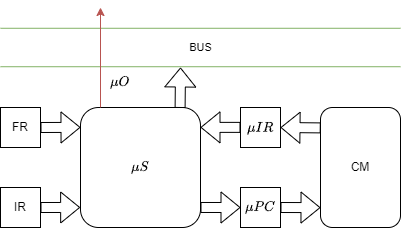
\includegraphics[width=0.8\textwidth]{media/mpcuarchitecture.png}
        \end{figure}
        \column{0.5\textwidth}
        \begin{itemize}
            \item \textbf{Control Memory $CM$}: Stores the microprogram (microinstructions).
            \item \textbf{Micro-Sequencer $\mu S$}: Fetches microinstructions from the control memory.
            \item \textbf{Micro-instruction Register $\mu IR$}: Stores the current microinstruction.
            \item \textbf{Micro-instruction Program Counter $\mu PC$}: Keeps track of the current microinstruction.
        \end{itemize}
    \end{columns}
    \note{
        The microprogrammed control unit consists of several key components:
        the control memory, micro-sequencer, micro-instruction register,
        and micro-instruction program counter.
        These components work together to fetch, store, and execute
        the microinstructions that generate control signals.
    }
\end{frame}

% Slide 7: Advantages of Microprogrammed Control Units
\begin{frame}
    \frametitle{Advantages of Microprogrammed Control Units}
    \begin{itemize}
        \item \textbf{Flexibility}: Easy to update; modifying control
        logic only requires updating the microprogram.
        \item \textbf{Simplicity}: Simplifies the design for CPUs
        with complex instruction sets.
        \item \textbf{Debugging}: Easier to debug because the logic is in the microcode.
        \item \textbf{Instruction Set Expansion}: Allows for adding new instructions
        \item \textbf{Less Hardware}: Requires less hardware than hardwired control units.
        \item \textbf{Emulates diffrent ISAs}: Can emulate any ISA.
    \end{itemize}
    \note{
        Microprogrammed control units are especially valuable in complex instruction
        set computers (CISC) due to their flexibility.
        Updating microinstructions is easier than changing hardware,
        which makes adding new instructions or optimizing existing ones simpler.
    }
\end{frame}

% Slide 7: Advantages of Microprogrammed Control Units
\begin{frame}
    \frametitle{Advantages of Microprogrammed Control Units}
    \begin{itemize}
        \item \textbf{Flexibility}: Easily updated by changing the microprogram.
        \item \textbf{Simplicity in Design}: Streamlines complex instruction set implementations.
        \item \textbf{Debugging Ease}: Centralized control logic simplifies error detection.
        \item \textbf{ISA Expansion}: Easily add new instructions.
        \item \textbf{Hardware Minimization}: Requires less control-specific hardware.
        \item \textbf{ISA Emulation}: Capable of emulating various instruction sets.
    \end{itemize}
    \note{
        Microprogrammed control units are highly flexible and easier to modify
        than hardwired units. This is especially beneficial in complex instruction
        set computers (CISC), where frequent updates are needed. Debugging is
        also simplified as the control logic is within the microprogram.
    }
\end{frame}

% Slide 8: Disadvantages of Microprogrammed Control Units
\begin{frame}
    \frametitle{Disadvantages of Microprogrammed Control Units}
    \begin{itemize}
        \item \textbf{Speed}: Slower than hardwired units due to microinstruction fetches.
        \item \textbf{Memory Requirements}: Additional memory required for microprogram storage.
    \end{itemize}
    \note{
        The primary downside of microprogrammed control units is their slower
        execution speed, as control signals must be fetched from memory.
        There's also memory overhead, as the microprogram must be stored
        separately from other data.
    }
\end{frame}

% Slide 9: Key Differences Between Control Units
\begin{frame}[fragile]
    \frametitle{Key Differences Between Control Units}
    \begin{table}
        \resizebox{0.9\textwidth}{!}{%
            \begin{tabular}{|c|c|c|c|}
                \hline
                \textbf{Feature} & \textbf{Unpipelined Hardwired} & \textbf{Microprogrammed} & \textbf{Pipelined Hardwired} \\
                \hline
                Control Signal Generation & Combinational Logic & Microinstructions & Combinational Logic \\
                \hline
                Flexibility & Low & High & Low \\
                \hline
                Best For & RISC & CISC & RISC/CISC \\
                \hline
                Memory Usage & No extra memory & Requires microprogram memory & Requires intermediate storage  \\
                \hline
                CPI & 1 & >1 & 1 \\
                \hline
                Cycle Time & Longer & Shorter (sequential) & Short (parallel)\\
                \hline
            \end{tabular}
        }
    \end{table}
    \note{
        This summary table contrasts each type of control unit across factors like flexibility,
        memory usage, and cycle time. Pipelined hardwired units,
        though similar to unpipelined ones in logic, can achieve lower cycle times
        due to parallelism.
    }
\end{frame}

\section{Implementation}
\begin{frame}
    \frametitle{Implementation for Lab CPU}
    \textbf{Type of interrupts:}
    \begin{itemize}
        \item Internal interrupts (non-maskable):
        \begin{itemize}
            \item ALU overflow
            \item Software interrupt through the \texttt{INT} instruction
        \end{itemize}
        \item External non-maskable interrupts:
        \begin{itemize}
            \item Lack of Voltage (Power Off)
            \item Special hardware line \texttt{cinm}
        \end{itemize}
        \item External maskable interrupts:
        \begin{itemize}
            \item 8 IO deivce interrupts
            \item Special hardware line \texttt{cintr} for all.
        \end{itemize}
    \end{itemize}
\end{frame}

\begin{frame}
    \frametitle{Implementation of IVT}
    \begin{table}[]
        \resizebox{0.9\textwidth}{!}{%
            \begin{tabular}{|c|c|c|}
                \hline
                \textbf{Address} & \textbf{Name} & \textbf{Type} \\ \hline
                0x0 & Reserved  & \multirow{3}{*}{Internal Interrupt} \\ \cline{1-2}
                0x1 & Software Interrupt (INT) & \\ \cline{1-2}
                0x2 & ALU Overflow & \\ \hline
                0x3 & Lack of Voltage (Power Off) & External Non-Maskable Interrupt \\ \hline
                0x4 & Level 0 & \multirow{8}{*}{External Maskable Interrupt} \\ \cline{1-2}
                0x5 & Level 1 & \\ \cline{1-2}
                0x6 & Level 2 & \\ \cline{1-2}
                0x7 & Level 3 & \\ \cline{1-2}
                0x8 & Level 4 & \\ \cline{1-2}
                0x9 & Level 5 & \\ \cline{1-2}
                0xA & Level 6 & \\ \cline{1-2}
                0xB & Level 7 & \\ \hline
            \end{tabular}
        }
    \end{table}
    \note{
    }

\end{frame}

\begin{frame}
    \frametitle{Interupt Instructions}
    The FR (Flag Register) will have a new bit \texttt{I} which will be used to enable or disable interrupts.
    The following instructions will be added:
    \begin{itemize}
        \item \texttt{EI} - Enable interrupts (sei)
        \item \texttt{DI} - Disable interrupts (cli)
        \item \texttt{INT} - Genrate software interrupt
        \item \texttt{RETI} - Return from interrupt
    \end{itemize}
\end{frame}

\begin{frame}
    \frametitle{Architecture}
    \begin{figure}
        \centering
        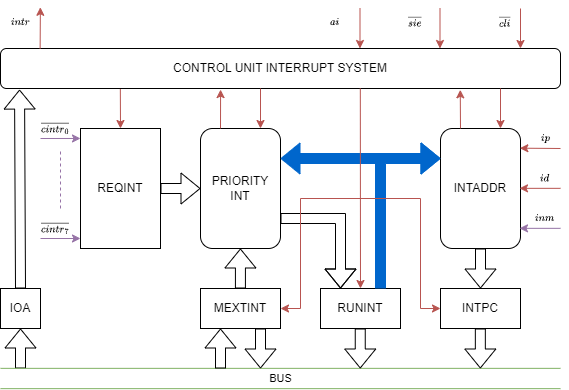
\includegraphics[width=0.8\textwidth]{media/isarchitecture.png}
    \end{figure}
\end{frame}

\begin{frame}
    \frametitle{Architecture Signals}
    \begin{itemize}
        \item $ip$ - Software Interrupt
        \item $id$ - ALU Overflow Interrupt
        \item $inm$ - external non-maskable interrupt (comes from $cinm$)
        \item $cintr_{i}$ - external maskable interrupt from device $i$
        \item $ai$ - external maskable interrupt active
        \item $intr$ - external maskable interrupt request to CPU
        \item $sie$/$cie$ - enable/disable external maskable interrupts
    \end{itemize}
\end{frame}

\begin{frame}
    \frametitle{Architecture Components}
    \begin{itemize}
        \item \texttt{REQINT} - Request external maskable interrupt register ($REQINT_{i} = 1$ means that the interrupt $i$ is requested)
        \item \texttt{MEXTINT} - Maskable external interrupt register ($MEXTINT_{i} = 1$ means that the interrupt $i$ is masked)
        \item \texttt{RUNINT} - Current running interrupts register ($RUNINT_{i} = 1$ means that the interrupt on level $i$ is running)
        \item \texttt{Priorrity INT} - Compute if the current interrupt has higher priority than the current running interrupt
        \item \texttt{INTADDR} - Compute the address of the ISR
        \item \texttt{INTPC} - The address for the current ISR
    \end{itemize}
\end{frame}

\begin{frame}
    \frametitle{External maskable interrupts Handling}
    \begin{enumerate}
        \item Verify for external maskable interrupt requests in the \texttt{REQINT} register.
        \item If there is one, verify if external maskable interrupts are enabled. (flag \texttt{I} in FR)
        \item If yes, filter the interrupts that are masked in the \texttt{MEXTINT} register.
        \item Find the highest priority interrupt that is not masked.
        \item Verify if it has higher priority than the current running interrupts in the \texttt{RUNINT} register:
        \item Send the interrupt to the CPU through the $intr$ signal.
        \item Wait for the CPU to acknowledge the interrupt. ($ai$ signal)
        \item Set the bit in the \texttt{RUNINT} register.
        \item Clear the bit in the \texttt{REQINT} register.
        \item Compute the address of the ISR and set the \texttt{INTPC} register.
    \end{enumerate}
\end{frame}

\begin{frame}
    \frametitle{External non-maskable interrupts Handling}
    \begin{enumerate}
        \item Verify for external non-maskable interrupt requests in the \texttt{inm} signal.
        \item Verify if there is no higher priority interrupt running.
        \item Compute the address of the ISR and set the \texttt{INTPC} register.
    \end{enumerate}
\end{frame}

\begin{frame}
    \frametitle{ALU Overflow Handling}
    \begin{enumerate}
        \item Verify for ALU overflow interrupt requests in the \texttt{id} signal.
        \item Verify if there is no higher priority interrupt running.
        \item Compute the address of the ISR and set the \texttt{INTPC} register.
        \item Inside the ISR, the CPU must clear the  overflow flag in the FR.
    \end{enumerate}
\end{frame}

\begin{frame}
    \frametitle{Software interrupts Handling}
    \begin{enumerate}
        \item Verify for software interrupt requests in the \texttt{ip} signal.
        \item There is no higher priority interrupt running.
        \item Compute the address of the ISR and set the \texttt{INTPC} register.
    \end{enumerate}
\end{frame}

\begin{frame}
    \frametitle{CPU acknowledge interrupts}
    \begin{enumerate}
        \item Save FR on the stack.
        \item Disable external maskable interrupts. (\texttt{EI} can be used to enable them back inside ISR)
        \item Save the current PC on the stack.
        \item Run the jump instruction from the \texttt{INTPC} register address.
    \end{enumerate}
\end{frame}

% \begin{frame}
%     \frametitle{Exam Questions}
%     Template: Having the following values in the registers at time 0,
%     interrupts requested with the time of the request and the type of the interrupt,
%     and how much time the CPU will take to handle every type of interrupt,
%     which is the order of the interrupts that will be handled by the CPU?
% \end{frame}


% \begin{frame}
%     \frametitle{Exam Questions}
%     \begin{table}[]
%         \begin{tabular}{|c|c|c|c|}
%             \hline
%             \texttt{REQINT} & \texttt{MEXTINT} & \texttt{RUNINT} & \texttt{FR} \\ \hline
%             0x00 & 0x00 & 0x00 & 0x00 \\ \hline
%         \end{tabular}
%     \end{table}

%     \begin{table}[]
%         \begin{tabular}{|c|c|c|c|}
%             \hline
%             Cycles from time 0 & Type of Request & Name \\ \hline
%             10 & External Maskable Interupt Level 5 & A \\ \hline
%             30 & External Maskable Interupt Level 3 & B \\ \hline
%             50 & External Maskable Interupt Level 7 & C \\ \hline
%             60 & External Maskable Interupt Level 1 & D \\ \hline
%             100 & External Non-Maskable Interupt & E \\ \hline
%             140 & ALU Overflow & F \\ \hline
%             150 & Software Interupt & G \\ \hline
%         \end{tabular}
%     \end{table}
% \end{frame}



% \begin{frame}
%     \frametitle{Exam Questions}
%     \begin{table}
%         \begin{tabular}{|c|c|c|c|}
%             \hline
%             Type of Request & Cycle to handle \\ \hline
%             External Maskable Interupt Level 0 & 30 \\ \hline
%             External Maskable Interupt Level 1 & 20 \\ \hline
%             External Maskable Interupt Level 2 & 10 \\ \hline
%             External Maskable Interupt Level 3 & 40 \\ \hline
%             External Maskable Interupt Level 4 & 20 \\ \hline
%             External Maskable Interupt Level 5 & 30 \\ \hline
%             External Maskable Interupt Level 6 & 10 \\ \hline
%             External Maskable Interupt Level 7 & 20 \\ \hline
%             External Non-Maskable Interupt & 5 \\ \hline
%             ALU Overflow & 10 \\ \hline
%             Software Interupt & 10 \\ \hline
%         \end{tabular}
%     \end{table}
% \end{frame}



% \begin{frame}
%     \frametitle{Exam Questions}
% \end{frame}

\section{Minimal microinstruction coding}
\begin{frame} 
    \frametitle{Engineering Minimal Micro-instruction Coding}
    \begin{itemize} 
        \item The problem is NP-complete.
        \item Goal: Minimize the word size of micro-instructions while
        considering ROM memory constraints ($2^n$ sizes).
        \item Using mono-phase micro-instructions.
    \end{itemize}
\end{frame}

\begin{frame}
    \frametitle{Problem Definition}
    \begin{itemize}
        \item Define micro-operation: $\mu O_{i}$.
        \item Define microinstruction: $\mu I_{i} = \{ \mu O_{0}, \mu O_{1}, \ldots, \mu O_{|I_{i}|} \}$.
        \item Set of unique micro-instructions in a program: $\mu P(\mu I) = \{\mu I_{0}, \mu I_{1}, \ldots, \mu I_{|\mu P(\mu I)|}\}$.
        \item Set of micro-operations in a program: $\mu P(\mu O) = \{\mu O_{0}, \mu O_{1}, \ldots, \mu O_{|\mu P(\mu O)|}\}$.
    \end{itemize}
\end{frame}

\begin{frame}
    \frametitle{Compatible Class of Micro-operations}
    \begin{itemize}
        \item Micro-operations $\mu O_{i}$ and $\mu O_{j}$ are compatible if $\forall \mu I_{k} \in \mu P(\mu I),
        \text{ if } \mu O_{i} \in \mu I_{k} \text{ than } \mu O_{j} \notin \mu I_{k}$.
        (do not execute in parallel).
        \item Compatible class: $CC(\mu O_{i}) = \{\mu O_{j} \in \mu P(\mu O)
         \ | \ \mu O_{i} \text{ and } \mu O_{j} \text{ are compatible}\}$.
        \item Maximum compatible class: $MCC(\mu O_{i}) = \{ CC(\mu O_{i})
         \ | \forall  \mu O_{j} \notin CC(\mu O_{i}) \text{ than }
         \exists \mu O_{k} \in CC(\mu O_{i}) \text{ and }
         \exists \mu I_{p} \in \mu P(\mu I) \text{, so }
         \mu O_{j} \in \mu I_{p} \text{ and } \mu O_{k} \in  \mu I_{p} \}$.
    \end{itemize}
\end{frame}

\begin{frame}
    \frametitle{Cost of Compatible Class}
    \begin{itemize}
        \item Cost of a compatible class: $C(CC(\mu O_{i})) = [\log_{2}(|CC(\mu O_{i})| + 1)]$.
        \item Total cost of a microinstruction: $C(\mu I) = \sum_{i=0}^{k} C(CC_{i})$,
        where $k$ is the number of compatible classes.
        \item Each compatible class corresponds to a field in the microinstruction.
    \end{itemize}
\end{frame}

\begin{frame}
    \frametitle{Approximate Minimal Coding Algorithm}
    \begin{itemize}
        \item Identify all Maximum Compatible Classes $MCC(\mu O_{i})$.
        \item Select a set of $MCC(\mu O_{i})$ to minimize $C(\mu I)$.
    \end{itemize}
\end{frame}

\begin{frame}
    \frametitle{Incompatible Classes}
    \begin{itemize}
        \item Incompatible class: $IC(\mu O_{i}) = \{ \mu O_{j} \in \mu P(\mu O) \ | \ \mu O_{i} \text{ and } \mu O_{j} \text{ are incompatible}\}$.
        \item Maximum incompatible class: $MIC(\mu O_{i}) = \{ IC(\mu O_{i}) \ | \forall  \mu O_{j} \notin IC(\mu O_{i}) \text{ than } \exists \mu O_{k} \in IC(\mu O_{i}) \text{ and } \exists \mu I_{p} \in \mu P(\mu I) \text{, so } \mu O_{j} \in \mu I_{p} \text{ and } \mu O_{k} \in  \mu I_{p} \}$.
        \item Associated maximum compatible class $AMCC(\mu O_{j}) = \{ MCC(\mu O_{j}) \ | \ \mu O_{j} \in IC(\mu O_{i})\}$.
    \end{itemize}
    \note{
    }
\end{frame}

\begin{frame}
    \frametitle{Algorithm Properties}
    \begin{itemize}
        \item $\forall MIC(\mu O_{i}) \text{ than } \bigcup_{\mu O_{j} \in MIC(\mu O_{i})} AMCC(\mu O_{j}) = \mu P(\mu O)$.
        \item $\forall MIC(\mu O_{i}) \text{ and } k < |MIC(\mu O_{i}) | \text{ than } \bigcap_{0 < i < k} MCC_{i} \neq \mu P(\mu O)$.
    \end{itemize}
    \note{
        The first condition proof is: $\exists \mu O_{k} \in \mu P(\mu O) \text{ so } \mu O_{k} \notin MIC(\mu O_{i}) \text{ and } \mu O_{k} \notin  \bigcup_{\mu O_{j} \in MIC(\mu O_{i})} AMCC(\mu O_{j})$,
        than $\mu O_{k}$ is incompatible with every micro-operation in $ MIC(\mu O_{i})$, false, because is the maximum incompatible class.

        Second condition proof is: a compatible class can contain only one micro-operation from a maximum incompatible class.
    }
\end{frame}

\begin{frame}
    \frametitle{Cost Properties}
    \begin{itemize}
        \item If $\mu P(\mu O)$ is partitioned in $q$ fields, the minimum cost is when $q-1$ fileds represents each one micro-operation and the last field represents the rest of the micro-operations.
        \item There is not solution of $q+h$ fields whith lower cost than a solution with $q$ fields.
    \end{itemize}
\end{frame}

\begin{frame}
    \frametitle{Algorithm Steps}
    \begin{enumerate}
        \item Find all the maximum incompatible classes $MIC(\mu O_{i})$.
        \item Select the largest $MIC(\mu O_{i})$ by cardinality.
        \item Find the associated maximum compatible classes $AMCC(\mu O_{j})$.
        \item Create a table of micro-operations (columns) and maximum compatible classes (rows).
        \item Identify essential compatible classes (containing unique micro-operations).
        \item Remove essential compatible classes and reduce the table. (add them to the solution)
        \item Select a set of remaining classes to cover all operations at minimal cost.
    \end{enumerate}
\end{frame}

\begin{frame}
    \frametitle{Exam Questions}
    Template: Given the following set of micro-instruction $\mu P(\mu I)$, with every micro-instruction table of micro-operations $\mu P(\mu O)$ executed in the table. Compute the minimal microinstruction coding.

    Example:

    $\mu P(\mu I) = \{ \mu I_{0}, \mu I_{1}, \mu I_{2}, \mu I_{3}, \mu I_{4}, \mu I_{5}, \mu I_{6}\}$
    $\mu P(\mu O) = \{ \mu O_{0}, \mu O_{1}, \mu O_{2}, \mu O_{3}, \mu O_{4}, \mu O_{5}, \mu O_{6}, \mu O_{7}, \mu O_{8}, \mu O_{9}\}$.
    \begin{table}
        \resizebox{0.8\textwidth}{!}{%
        \begin{tabular}{|c|c|c|c|c|c|c|c|c|c|c|}
            \hline
            $\mu I$ & $\mu O_{0}$ & $\mu O_{1}$ & $\mu O_{2}$ & $\mu O_{3}$ & $\mu O_{4}$ & $\mu O_{5}$ & $\mu O_{6}$ & $\mu O_{7}$ & $\mu O_{8}$ & $\mu O_{9}$ \\
            \hline
            \hline
            $\mu I_{0}$ & 1 & 1 & 0 & 1 & 0 & 0 & 0 & 0 & 0 & 0 \\ \hline
            $\mu I_{1}$ & 1 & 0 & 1 & 0 & 1 & 0 & 0 & 0 & 0 & 0 \\ \hline
            $\mu I_{2}$ & 0 & 1 & 0 & 0 & 0 & 1 & 0 & 1 & 1 & 0 \\ \hline
            $\mu I_{3}$ & 0 & 0 & 0 & 1 & 1 & 0 & 1 & 1 & 0 & 0 \\ \hline
            $\mu I_{4}$ & 0 & 0 & 1 & 1 & 1 & 1 & 1 & 0 & 0 & 0 \\ \hline
            $\mu I_{5}$ & 0 & 0 & 0 & 0 & 0 & 1 & 0 & 0 & 1 & 1 \\ \hline
            $\mu I_{6}$ & 0 & 0 & 0 & 0 & 0 & 0 & 1 & 0 & 0 & 1 \\ \hline
        \end{tabular}%
        }
    \end{table}
\end{frame}

\begin{frame}
    \frametitle{Solution - Table of incompatible operations}
    \begin{table}
        \resizebox{0.8\textwidth}{!}{%
            \begin{tabular}{|c|c|c|c|c|c|c|c|c|c|c|c|}
                \hline
                $\mu O$ & $\mu O_{0}$ & $\mu O_{1}$ & $\mu O_{2}$ & $\mu O_{3}$ & $\mu O_{4}$ & $\mu O_{5}$ & $\mu O_{6}$ & $\mu O_{7}$ & $\mu O_{8}$ & $\mu O_{9}$ \\ \hline
                $\mu O_{0}$ & 1 & 1 & 1 & 1 & 1 & 0 & 0 & 0 & 0 & 0 \\ \hline
                $\mu O_{1}$ & 1 & 1 & 0 & 1 & 0 & 1 & 0 & 1 & 1 & 0 \\ \hline
                $\mu O_{2}$ & 1 & 0 & 1 & 1 & 1 & 1 & 1 & 0 & 0 & 0 \\ \hline
                $\mu O_{3}$ & 1 & 1 & 1 & 1 & 1 & 1 & 1 & 1 & 0 & 0 \\ \hline
                $\mu O_{4}$ & 1 & 0 & 1 & 1 & 1 & 1 & 1 & 1 & 0 & 0 \\ \hline
                $\mu O_{5}$ & 0 & 1 & 1 & 1 & 1 & 1 & 1 & 1 & 1 & 1 \\ \hline
                $\mu O_{6}$ & 0 & 0 & 1 & 1 & 1 & 1 & 1 & 1 & 0 & 1 \\ \hline
                $\mu O_{7}$ & 0 & 1 & 0 & 1 & 1 & 1 & 1 & 1 & 1 & 0 \\ \hline
                $\mu O_{8}$ & 0 & 1 & 0 & 0 & 0 & 1 & 0 & 1 & 1 & 1 \\ \hline
                $\mu O_{9}$ & 0 & 0 & 0 & 0 & 0 & 1 & 1 & 0 & 1 & 1 \\ \hline
            \end{tabular}%
        }
    \end{table}
\end{frame}

\begin{frame}
    \frametitle{Solution - Maximum incompatible classes}
    \begin{table}
        \resizebox{0.8\textwidth}{!}{%
            \begin{tabular}{|c|c|c|c|c|c|c|c|c|c|c|c|}
                \hline
                $MIC$ & $\mu O_{0}$ & $\mu O_{1}$ & $\mu O_{2}$ & $\mu O_{3}$ & $\mu O_{4}$ & $\mu O_{5}$ & $\mu O_{6}$ & $\mu O_{7}$ & $\mu O_{8}$ & $\mu O_{9}$ \\ \hline
                $MIC(\mu O_{0})$ & 1 & 1 & 0 & 1 & 0 & 0 & 0 & 0 & 0 & 0 \\ \hline
                $MIC(\mu O_{1})$ & 1 & 0 & 1 & 1 & 1 & 0 & 0 & 0 & 0 & 0 \\ \hline
                $MIC(\mu O_{2})$ & 0 & 1 & 0 & 1 & 0 & 1 & 0 & 1 & 0 & 0 \\ \hline
                $MIC(\mu O_{3})$ & 0 & 1 & 0 & 0 & 0 & 1 & 0 & 1 & 1 & 0 \\ \hline
                $MIC(\mu O_{4})$ & 0 & 0 & 1 & 1 & 1 & 1 & 1 & 0 & 0 & 0 \\ \hline
                $MIC(\mu O_{5})$ & 0 & 0 & 0 & 1 & 1 & 1 & 1 & 1 & 0 & 0 \\ \hline
                $MIC(\mu O_{6})$ & 0 & 0 & 0 & 0 & 0 & 1 & 1 & 0 & 0 & 1 \\ \hline
                $MIC(\mu O_{7})$ & 0 & 0 & 0 & 0 & 0 & 1 & 0 & 0 & 1 & 1 \\ \hline
            \end{tabular}%
        }
    \end{table}
    \note{
        To make incompatible classes we choose micro-operation from the table of incompatible operations and AND their rows.
        If there is a 1 in the result that micro-operation is incompatible with the other micro-operations and is can be
        added to the incompatible class. If there are only 0s in the result than the current set of micro-operations is a maximum incompatible class.
    }
\end{frame}

\begin{frame}
    \frametitle{Solution - Maximum compatible classes}
    \begin{table}
        \resizebox{0.8\textwidth}{!}{%
            \begin{tabular}{|c|c|c|c|c|c|c|c|c|c|c|}
                \hline
                $MCC$ & $\mu O_{0}$ & $\mu O_{1}$ & $\mu O_{2}$ & $\mu O_{3}$ & $\mu O_{4}$ & $\mu O_{5}$ & $\mu O_{6}$ & $\mu O_{7}$ & $\mu O_{8}$ & $\mu O_{9}$ \\ \hline
                $MCC_{0}$ & 1 & 0 & 0 & 0 & 0 & 1 & 0 & 0 & 0 & 0 \\ \hline
                $MCC_{1}$ & 1 & 0 & 0 & 0 & 0 & 0 & 1 & 0 & 1 & 0 \\ \hline
                $MCC_{2}$ & 1 & 0 & 0 & 0 & 0 & 0 & 0 & 1 & 0 & 1 \\ \hline
                $MCC_{3}$ & 0 & 1 & 1 & 0 & 0 & 0 & 0 & 0 & 0 & 1 \\ \hline
                $MCC_{4}$ & 0 & 1 & 0 & 0 & 1 & 0 & 0 & 0 & 0 & 1 \\ \hline
                $MCC_{5}$ & 0 & 1 & 0 & 0 & 0 & 0 & 1 & 0 & 0 & 0 \\ \hline
                $MCC_{6}$ & 0 & 0 & 1 & 0 & 0 & 0 & 0 & 1 & 0 & 1 \\ \hline
                $MCC_{7}$ & 0 & 0 & 1 & 0 & 0 & 0 & 0 & 0 & 1 & 0 \\ \hline
                $MCC_{8}$ & 0 & 0 & 0 & 1 & 0 & 0 & 0 & 0 & 1 & 0 \\ \hline
                $MCC_{9}$ & 0 & 0 & 0 & 1 & 0 & 0 & 0 & 0 & 0 & 1 \\ \hline
                $MCC_{10}$ & 0 & 0 & 0 & 0 & 1 & 0 & 0 & 0 & 1 & 0 \\ \hline
            \end{tabular}%
        }
    \end{table}
\end{frame}

\begin{frame}
    \frametitle{Solution - Associated maximum compatible classes}
    Select the maximum incompatible class with the biggest cardinality. In this case is $MIC(\mu O_{4})$ or $MIC(\mu O_{5})$.
    Let's choose $MIC(\mu O_{5})$.
    $AMCC(\mu O_{i} \in MIC(\mu O_{5})) = \{ MCC_{0}, MCC_{1}, MCC_{2}, MCC_{4}, MCC_{5}, MCC_{6}, MCC_{8}, MCC_{9}, MCC_{10}\}$
    
    \begin{table}
        \resizebox{0.8\textwidth}{!}{%
            \begin{tabular}{|c|c|c|c|c|c|c|c|c|c|c|}
                \hline
                $MCC$ & $\mu O_{0}$ & $\mu O_{1}$ & $\mu O_{2}$ & $\mu O_{3}$ & $\mu O_{4}$ & $\mu O_{5}$ & $\mu O_{6}$ & $\mu O_{7}$ & $\mu O_{8}$ & $\mu O_{9}$ \\ \hline
                $MCC_{0}$ & 1 & 0 & 0 & 0 & 0 & 1 & 0 & 0 & 0 & 0 \\ \hline
                $MCC_{1}$ & 1 & 0 & 0 & 0 & 0 & 0 & 1 & 0 & 1 & 0 \\ \hline
                $MCC_{2}$ & 1 & 0 & 0 & 0 & 0 & 0 & 0 & 1 & 0 & 1 \\ \hline
                $MCC_{4}$ & 0 & 1 & 0 & 0 & 1 & 0 & 0 & 0 & 0 & 1 \\ \hline
                $MCC_{5}$ & 0 & 1 & 0 & 0 & 0 & 0 & 1 & 0 & 0 & 0 \\ \hline
                $MCC_{6}$ & 0 & 0 & 1 & 0 & 0 & 0 & 0 & 1 & 0 & 1 \\ \hline
                $MCC_{8}$ & 0 & 0 & 0 & 1 & 0 & 0 & 0 & 0 & 1 & 0 \\ \hline
                $MCC_{9}$ & 0 & 0 & 0 & 1 & 0 & 0 & 0 & 0 & 0 & 1 \\ \hline
                $MCC_{10}$ & 0 & 0 & 0 & 0 & 1 & 0 & 0 & 0 & 1 & 0 \\ \hline
            \end{tabular}%
        }
    \end{table}
\end{frame}

\begin{frame}
    \frametitle{Solution - Essential compatible classes}
    Select the essential compatible classes. In this case $MCC_{0}$ and $MCC_{6}$.
    $S = \{MCC_{0}, MCC_{6}\}$.
    % \begin{table}
    %     \resizebox{0.8\textwidth}{!}{%
    %         \begin{tabular}{|c|c|c|c|c|c|c|c|c|c|c|}
    %             \hline
    %             $MCC$ & $\mu O_{0}$ & $\mu O_{1}$ & $\mu O_{2}$ & $\mu O_{3}$ & $\mu O_{4}$ & $\mu O_{5}$ & $\mu O_{6}$ & $\mu O_{7}$ & $\mu O_{8}$ & $\mu O_{9}$ \\ \hline
    %             $MCC_{1}$ & 1 & 0 & 0 & 0 & 0 & 0 & 1 & 0 & 1 & 0 \\ \hline
    %             $MCC_{2}$ & 1 & 0 & 0 & 0 & 0 & 0 & 0 & 1 & 0 & 1 \\ \hline
    %             $MCC_{4}$ & 0 & 1 & 0 & 0 & 1 & 0 & 0 & 0 & 0 & 1 \\ \hline
    %             $MCC_{5}$ & 0 & 1 & 0 & 0 & 0 & 0 & 1 & 0 & 0 & 0 \\ \hline
    %             $MCC_{8}$ & 0 & 0 & 0 & 1 & 0 & 0 & 0 & 0 & 1 & 0 \\ \hline
    %             $MCC_{9}$ & 0 & 0 & 0 & 1 & 0 & 0 & 0 & 0 & 0 & 1 \\ \hline
    %             $MCC_{10}$ & 0 & 0 & 0 & 0 & 1 & 0 & 0 & 0 & 1 & 0 \\ \hline
    %         \end{tabular}%
    %     }
    % \end{table}
    \begin{table}
        \resizebox{0.8\textwidth}{!}{%
            \begin{tabular}{|c|c|c|c|c|c|c|}
                \hline
                $MCC$ & $\mu O_{1}$ & $\mu O_{3}$ & $\mu O_{4}$ & $\mu O_{6}$ & $\mu O_{8}$ \\ \hline
                $MCC_{1}$ & 0 & 0 & 0 & 1 & 1 \\ \hline
                $MCC_{2}$ & 0 & 0 & 0 & 0 & 0 \\ \hline
                $MCC_{4}$ & 1 & 0 & 1 & 0 & 0 \\ \hline
                $MCC_{5}$ & 1 & 0 & 0 & 1 & 0 \\ \hline
                $MCC_{8}$ & 0 & 1 & 0 & 0 & 1 \\ \hline
                $MCC_{9}$ & 0 & 1 & 0 & 0 & 0 \\ \hline
                $MCC_{10}$ & 0 & 0 & 1 & 0 & 1 \\ \hline
            \end{tabular}%
        }
    \end{table}
    \note{
        The essential compatible classes are the ones that contain a micro-operation that is not in any other compatible class.
        Remove the essential compatible classes from the table and add them to the solution set.
     }
\end{frame}

\begin{frame}
    \frametitle{Solution - Remaining compatible classes}
    $MCC_{2}$ and $MCC_{9}$ does not contain any micro-operation that is not in any other compatible class. So we can remove them from the table.   
    \begin{table}
        \resizebox{0.8\textwidth}{!}{%
            \begin{tabular}{|c|c|c|c|c|c|c|}
                \hline
                $MCC$ & $\mu O_{1}$ & $\mu O_{3}$ & $\mu O_{4}$ & $\mu O_{6}$ & $\mu O_{8}$ \\ \hline
                $MCC_{1}$ & 0 & 0 & 0 & 1 & 1 \\ \hline
                $MCC_{4}$ & 1 & 0 & 1 & 0 & 0 \\ \hline
                $MCC_{5}$ & 1 & 0 & 0 & 1 & 0 \\ \hline
                $MCC_{8}$ & 0 & 1 & 0 & 0 & 1 \\ \hline
                $MCC_{10}$ & 0 & 0 & 1 & 0 & 1 \\ \hline
            \end{tabular}%
        }
    \end{table}
    This makes $MCC_{8}$ an essential compatible class. Remove it from the table and add it to the solution set.
    $S = \{MCC_{0}, MCC_{6}, MCC_{8}\}$.
\end{frame}

\begin{frame}
    \frametitle{Solution - Remaining compatible classes}
    \begin{table}
        \resizebox{0.8\textwidth}{!}{%
            \begin{tabular}{|c|c|c|c|c|c|c|}
                \hline
                $MCC$ & $\mu O_{1}$ & $\mu O_{4}$ & $\mu O_{6}$ \\ \hline
                $MCC_{1}$ & 0 & 0 & 1 \\ \hline
                $MCC_{4}$ & 1 & 1 & 0 \\ \hline
                $MCC_{5}$ & 1 & 0 & 1 \\ \hline
                $MCC_{10}$ & 0 & 1 & 0 \\ \hline
            \end{tabular}%
        }
    \end{table}
    The possible additions solution sets are: $\{MCC_{1}, MCC_{4}\}$, $\{MCC_{4}, MCC_{5}\}$, $\{MCC_{5}, MCC_{10}\}$.
    The possible sollution sets are: $\{MCC_{0}, MCC_{6}, MCC_{8}, MCC_{1}, MCC_{4}\}$, $\{MCC_{0}, MCC_{6}, MCC_{8}, MCC_{4}, MCC_{5}\}$, $\{MCC_{0}, MCC_{6}, MCC_{8}, MCC_{5}, MCC_{10}\}$.
\end{frame}

\begin{frame}
    \frametitle{Solution - Minimal microinstruction coding}
    The table with all micro operations and the selected compatible classes.
    \begin{table}
        \resizebox{0.8\textwidth}{!}{%
            \begin{tabular}{|c|c|c|c|c|c|c|c|c|c|c|c|}
                \hline
                $MCC$ & $\mu O_{0}$ & $\mu O_{1}$ & $\mu O_{2}$ & $\mu O_{3}$ & $\mu O_{4}$ & $\mu O_{5}$ & $\mu O_{6}$ & $\mu O_{7}$ & $\mu O_{8}$ & $\mu O_{9}$ & $|MCC|$ \\ \hline
                $MCC_{0}$ & 1 & 0 & 0 & 0 & 0 & 1 & 0 & 0 & 0 & 0 & 2\\ \hline
                $MCC_{1}$ & 1 & 0 & 0 & 0 & 0 & 0 & 1 & 0 & 1 & 0 & 3\\ \hline
                $MCC_{4}$ & 0 & 1 & 0 & 0 & 1 & 0 & 0 & 0 & 0 & 1 & 3\\ \hline
                $MCC_{5}$ & 0 & 1 & 0 & 0 & 0 & 0 & 1 & 0 & 0 & 0 & 2\\ \hline
                $MCC_{6}$ & 0 & 0 & 1 & 0 & 0 & 0 & 0 & 1 & 0 & 1 & 3\\ \hline
                $MCC_{8}$ & 0 & 0 & 0 & 1 & 0 & 0 & 0 & 0 & 1 & 0 & 2\\ \hline
                $MCC_{10}$ & 0 & 0 & 0 & 0 & 1 & 0 & 0 & 0 & 1 & 0 & 2\\ \hline
            \end{tabular}%
        }
    \end{table}
    Order the maximum compatible classes in the solution set by their cardinality.
\end{frame}


\begin{frame}
    \frametitle{Solution - Minimal microinstruction coding}
    The cost for the solutions are:
    \begin{itemize}
        \item $C(S_{0}) = \{ (\mu O_{2}, \mu O_{7}, \mu O_{9}), (\mu O_{0}, \mu O_{6}, \mu O_{8}), (\mu O_{1}, \mu O_{4}), (\mu O_{3}), (\mu O_{5}) \} = 8$
        \item $C(S_{1}) = \{ (\mu O_{2}, \mu O_{7}, \mu O_{9}), (\mu O_{0}, \mu O_{5}), (\mu O_{1}, \mu O_{6}), (\mu O_{8}, \mu O_{3}), (\mu O_{4})  \} = 9$
        \item $C(S_{2}) = \{ (\mu O_{2}, \mu O_{7}, \mu O_{9}), (\mu O_{1}, \mu O_{6}), (\mu O_{0}, \mu O_{5}), (\mu O_{3}, \mu O_{8}), (\mu O_{4}) \} = 9$
    \end{itemize}
    The minimal microinstruction coding is $S_{0} = \{MCC_{0}, MCC_{6}, MCC_{8}, MCC_{1}, MCC_{4}\}$.
\end{frame}



\section{Q\&A}
\begin{frame}
\end{frame}

%\begin{frame}
%\frametitle{Table of Contents}
%\tableofcontents
%\end{frame}


\end{document}